%%%%%%%%%%%%%%%%%%%%%%%%%%%%%%%%%%%%%%%%%%%%%%%
\chapter{Introduction and Motivation} \label{chap:introduction}
%%%%%%%%%%%%%%%%%%%%%%%%%%%%%%%%%%%%%%%%%%%%%%%

\section{Era of Computing and Wireless Communication}
Ability of computing 




In 1948, scientists at the Bell Laboratories achieved two landmark research results:
Claude E.~Shannon published his paper \emph{A mathematical theory of communication} and John Bardeen, Walter Brattain and William Shockley announced the invention of the \emph{transistor effect}.

\cite{Arikan}

A binomial distribution is shown in %Figure~\ref{fig:coin_bino}.

%\begin{figure}[!htb]
%    \centering
%    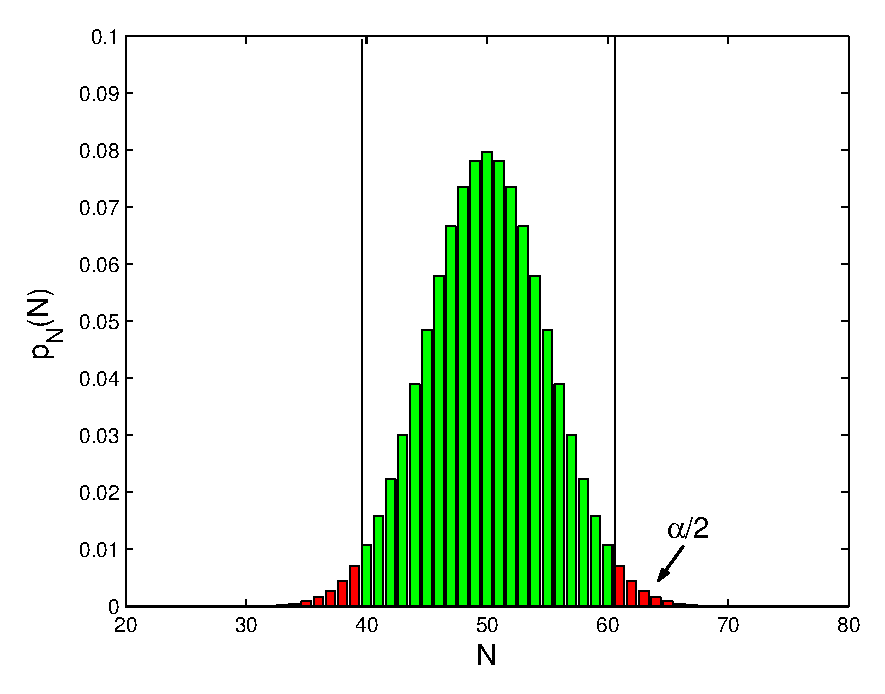
\includegraphics[width=0.8\textwidth]{./figures/coin_bino.eps}
%    \caption{PDF $p_N(N)$ of the number N of times that the head side is up.}
%    \label{fig:coin_bino}
%\end{figure}

For further information, the reader is referred to~\cite{Cover}.\newline

Traditionally FEC chains are developed in hardware i.e FPGA’s or ASIC’s to achieve low latency and high throughput.
Development in FPGA/hardware requires more time and costly.
With recent advances in General Purpose Processors it is possible to achieve required latency and throughput with software implementations without custom hardware.
Software implementations are flexible and easy to maintain compared hardware implementations.

However algorithms need to be adopted/optimized to efficiently implement in software.

Recent advances in the modern processors such as SIMD units can be utilized to achieve low latency and high throughput.

\section{Software implementation}



\section*{Organization of the Thesis}
%Having described the overall problem and relevant motivation, in Chapter 2 we develop
%the necessary mathematical framework to study decentralized cooperation problem pre-
%cisely. In Chapter 3, we identify the achievable consistency quality distortion region and
%build the notion of correlated time sharing which allows isolated node cooperation. Us-
%ing the abstract ideas developed in Chapter 3, we specialize the cooperation problem for
%discrete alphabet sources, develop simple decentralized schemes and compare their per-
%formances in terms of achievable consistency and quality performances. Similar to which
%101.4. Relation to the Heegard-Berger Problem
%in Chapter 5, we study the decentralized cooperation problem for random variables over
%continuous alphabet sets, develop simple heuristic schemes to achieve cooperation and
%compare their performances through simulation